\documentclass{article}
\usepackage{amsmath}
\usepackage[top=2cm, left=2cm, right=1cm, bottom=2cm]{geometry}
\usepackage{fancyhdr}
\usepackage{graphicx}
\usepackage{longtable}

\usepackage{amsmath,amssymb}
\usepackage{iftex}
\ifPDFTeX
  \usepackage[T1]{fontenc}
  \usepackage[utf8]{inputenc}
  \usepackage{textcomp} % provide euro and other symbols
\else % if luatex or xetex
  \usepackage{unicode-math} % this also loads fontspec
  \defaultfontfeatures{Scale=MatchLowercase}
  \defaultfontfeatures[\rmfamily]{Ligatures=TeX,Scale=1}
\fi
\usepackage{lmodern}
\ifPDFTeX\else
  % xetex/luatex font selection
\fi
% Use upquote if available, for straight quotes in verbatim environments
\IfFileExists{upquote.sty}{\usepackage{upquote}}{}
\IfFileExists{microtype.sty}{% use microtype if available
  \usepackage[]{microtype}
  \UseMicrotypeSet[protrusion]{basicmath} % disable protrusion for tt fonts
}{}
\makeatletter
\@ifundefined{KOMAClassName}{% if non-KOMA class
  \IfFileExists{parskip.sty}{%
    \usepackage{parskip}
  }{% else
    \setlength{\parindent}{0pt}
    \setlength{\parskip}{6pt plus 2pt minus 1pt}}
}{% if KOMA class
  \KOMAoptions{parskip=half}}
\makeatother
\usepackage{xcolor}
\usepackage{longtable,booktabs,array}
\usepackage{calc} % for calculating minipage widths
% Correct order of tables after \paragraph or \subparagraph
\usepackage{etoolbox}
\makeatletter
\patchcmd\longtable{\par}{\if@noskipsec\mbox{}\fi\par}{}{}
\makeatother
% Allow footnotes in longtable head/foot
\IfFileExists{footnotehyper.sty}{\usepackage{footnotehyper}}{\usepackage{footnote}}
\makesavenoteenv{longtable}
\usepackage{graphicx}
\makeatletter
\def\maxwidth{\ifdim\Gin@nat@width>\linewidth\linewidth\else\Gin@nat@width\fi}
\def\maxheight{\ifdim\Gin@nat@height>\textheight\textheight\else\Gin@nat@height\fi}
\makeatother
% Scale images if necessary, so that they will not overflow the page
% margins by default, and it is still possible to overwrite the defaults
% using explicit options in \includegraphics[width, height, ...]{}
\setkeys{Gin}{width=\maxwidth,height=\maxheight,keepaspectratio}
% Set default figure placement to htbp
\makeatletter
\def\fps@figure{htbp}
\makeatother
\setlength{\emergencystretch}{3em} % prevent overfull lines
\providecommand{\tightlist}{%
}
\setcounter{secnumdepth}{-\maxdimen} % remove section numbering
\ifLuaTeX
  \usepackage{selnolig}  % disable illegal ligatures
\fi
\usepackage{bookmark}
\IfFileExists{xurl.sty}{\usepackage{xurl}}{} % add URL line breaks if available
\urlstyle{same}
\hypersetup{
  hidelinks,
  pdfcreator={LaTeX via pandoc}}


\begin{document}
\pagestyle{fancy}
\fancyhf{}
\lfoot{Test ID: 2048}
\rfoot{Page: \thepage}
\renewcommand{\footrulewidth}{0.4pt}

\begin{enumerate}
	\itemsep2em
	\item
	\begin{minipage}[t]{\linewidth}
		Let \(f(x)=\sqrt{x}\). What is the equation of the tangent line to \(f\)
at the point \((4,2)\)?


		\vspace{1em}

		\begin{enumerate}
		\setlength\itemsep{2em}
			\item  $y=-\frac{1}{2} x+3$ 
			\item  $y=\frac{1}{2} x$ 
			\item  $y=2 x-6$ 
			\item  $y=\frac{1}{4} x+1$ 
		\end{enumerate}
	\end{minipage}
	\item
	\begin{minipage}[t]{\linewidth}
		What is the derivative of \(s(t)=\sec \sqrt{t}\) ?


		\vspace{1em}

		\begin{enumerate}
		\setlength\itemsep{2em}
			\item  $\sec \frac{1}{2 \sqrt{t}} \tan \frac{1}{2 \sqrt{t}}$ 
			\item  $\frac{\sec \sqrt{t} \tan \sqrt{t}}{2 \sqrt{t}}$ 
			\item  $\sec \sqrt{t} \tan \sqrt{t}$ 
			\item  $\tan ^{2} \sqrt{t}$ 
		\end{enumerate}
	\end{minipage}
	\item
	\begin{minipage}[t]{\linewidth}
		If \(f, g\), and \(h\) are nonzero differentiable functions, then the
derivative of \(\frac{f g}{h}\) is


		\vspace{1em}

		\begin{enumerate}
		\setlength\itemsep{2em}
			\item  $\frac{f g^{\prime} h^{\prime}-f g h^{\prime}}{h^{2}}$ 
			\item  $\frac{f g h^{\prime}-f g^{\prime} h-f^{\prime} g h}{h^{2}}$ 
			\item  $\frac{f^{\prime} g h+f g^{\prime} h+f g h^{\prime}}{h^{2}}$ 
			\item  $\frac{f g^{\prime} h+f^{\prime} g h-f g h^{\prime}}{h^{2}}$ 
			\item  $\frac{f g^{\prime}+f^{\prime} g}{h^{\prime}}$ 
		\end{enumerate}
	\end{minipage}
	\item
	\begin{minipage}[t]{\linewidth}
		The line tangent to the curve \(y=\sqrt{16-x}\) at the point \((0,4)\)
has slope


		\vspace{1em}

		\begin{enumerate}
		\setlength\itemsep{2em}
			\item  4 
			\item  $1 / 8$ 
			\item  $-1 / 8$ 
			\item  -8 
			\item  8 
		\end{enumerate}
	\end{minipage}
	\item
	\begin{minipage}[t]{\linewidth}
		At what point(s) on the curve \(x^{2}-y^{2}+x=2\) is the tangent line
vertical?


		\vspace{1em}

		\begin{enumerate}
		\setlength\itemsep{2em}
			\item  $(-2,0)$ only 
			\item  $(1, \sqrt{2})$ only 
			\item  $(1,0)$ and $(-2,0)$ 
			\item  The tangent line is never vertical 
			\item  $(1,0)$ only 
		\end{enumerate}
	\end{minipage}
	\item
	\begin{minipage}[t]{\linewidth}
		If \(y=6 \cos (3 x)\) then what is \(y^{\prime}\) ?


		\vspace{1em}

		\begin{enumerate}
		\setlength\itemsep{2em}
			\item  $18 \sin (x)$ 
			\item  $18 \sin (3 x)$ 
			\item  $-18 \sin (3 x)$ 
			\item  $-6 \sin (3 x)$ 
		\end{enumerate}
	\end{minipage}
	\item
	\begin{minipage}[t]{\linewidth}
		What is the value of

\[
\lim _{\Delta x \rightarrow 0} \frac{2(x+\Delta x)^{2}-2 x^{2}}{\Delta x}
\]


		\vspace{1em}

		\begin{enumerate}
		\setlength\itemsep{2em}
			\item  $4 x$ 
			\item  4 
			\item  2 
			\item  Does not exist 
			\item  $2 x$ 
		\end{enumerate}
	\end{minipage}
	\item
	\begin{minipage}[t]{\linewidth}
		If \(w(t)=\sqrt{t^{2}-1}\) what is the value of \(w^{\prime}(4)\) ?


		\vspace{1em}

		\begin{enumerate}
		\setlength\itemsep{2em}
			\item  $\frac{2}{\sqrt{15}}$ 
			\item  $\frac{1}{\sqrt{15}}$ 
			\item  $\frac{1}{2 \sqrt{15}}$ 
			\item  $\frac{4}{\sqrt{15}}$ 
		\end{enumerate}
	\end{minipage}
	\item
	\begin{minipage}[t]{\linewidth}
		At which \(x\) value does the graph of \(y=3 x^{2}-10 x+15\) have a
horizontal tangent line?


		\vspace{1em}

		\begin{enumerate}
		\setlength\itemsep{2em}
			\item  $\frac{-3}{5}$ 
			\item  $\frac{5}{3}$ 
			\item  $\frac{-5}{3}$ 
			\item  $\frac{3}{5}$ 
		\end{enumerate}
	\end{minipage}
	\item
	\begin{minipage}[t]{\linewidth}
		Find \(\frac{d y}{d x}\) if \(x^{2}+4 x y+2 y^{2}=16\)


		\vspace{1em}

		\begin{enumerate}
		\setlength\itemsep{2em}
			\item  $\frac{-2(x+y)}{x+2 y}$ 
			\item  $\frac{-2(x+y)}{2 x+y}$ 
			\item  $\frac{-x+2 y}{x+y}$ 
			\item  $\frac{-x-2 y}{2 x+2 y}$ 
		\end{enumerate}
	\end{minipage}
	\item
	\begin{minipage}[t]{\linewidth}
		At which \(x\) value(s) does the graph of \(y=2 x^{3}-24 x+16\) have a
horizontal tangent line?


		\vspace{1em}

		\begin{enumerate}
		\setlength\itemsep{2em}
			\item  2 
			\item  1 
			\item  2 and -2 
			\item  1 and -1 
		\end{enumerate}
	\end{minipage}
	\item
	\begin{minipage}[t]{\linewidth}
		If \(h(x)=f\left(x^{2}+1\right)\) then which of the following is true?


		\vspace{1em}

		\begin{enumerate}
		\setlength\itemsep{2em}
			\item  $h^{\prime}(x)=f^{\prime}(2 x)$ 
			\item  $h^{\prime}(x)=2 x f^{\prime}(2 x)$ 
			\item  $h^{\prime}(x)=2 x f^{\prime}\left(x^{2}+1\right)$ 
			\item  $h^{\prime}(x)=f^{\prime}\left(x^{2}+1\right)$ 
		\end{enumerate}
	\end{minipage}
	\item
	\begin{minipage}[t]{\linewidth}
		If \(f(x)=10 x^{2}-5\), what is the average rate of change of \(f(x)\)
over the interval

\[
-1 \leq x \leq 2
\]


		\vspace{1em}

		\begin{enumerate}
		\setlength\itemsep{2em}
			\item  30 
			\item  20 
			\item  $\frac{20}{3}$ 
			\item  10 
		\end{enumerate}
	\end{minipage}
	\item
	\begin{minipage}[t]{\linewidth}
		If \(h(x)=f(x) g(x)\) and
\(f(5)=3, f^{\prime}(5)=-1, g(5)=-\frac{1}{2}, g^{\prime}(5)=2\), then
what is the value of \(h^{\prime}(5)\) ?


		\vspace{1em}

		\begin{enumerate}
		\setlength\itemsep{2em}
			\item  $\frac{13}{2}$ 
			\item  $-\frac{9}{2}$ 
			\item  $\frac{9}{2}$ 
			\item  -2 
		\end{enumerate}
	\end{minipage}
	\item
	\begin{minipage}[t]{\linewidth}
		If \(f(x)=\sin \left(x^{2}+1\right)\) then find \(f^{\prime \prime}(x)\)


		\vspace{1em}

		\begin{enumerate}
		\setlength\itemsep{2em}
			\item  $-4 x^{2} \sin \left(x^{2}+1\right)+2 \cos \left(x^{2}+1\right)$ 
			\item  $4 x^{2} \sin \left(x^{2}+1\right)-2 \cos \left(x^{2}+1\right)$ 
			\item  $-4 x^{2} \sin \left(x^{2}+1\right)-2 \cos \left(x^{2}+1\right)$ 
			\item  $4 x^{2} \sin \left(x^{2}+1\right)+2 \cos \left(x^{2}+1\right)$ 
		\end{enumerate}
	\end{minipage}
	\item
	\begin{minipage}[t]{\linewidth}
		The height (in feet) of a ball thrown vertically upward is given by

\[
s(t)=-16 t^{2}+32 t+64
\]

where \(t\) is in seconds. What is the velocity of the ball at time
\(t=3\) seconds?


		\vspace{1em}

		\begin{enumerate}
		\setlength\itemsep{2em}
			\item  $64 \mathrm{ft} / \mathrm{s}$ 
			\item  $-16 \mathrm{ft} / \mathrm{s}$ 
			\item  $16 \mathrm{ft} / \mathrm{s}$ 
			\item  $-64 \mathrm{ft} / \mathrm{s}$ 
		\end{enumerate}
	\end{minipage}
	\item
	\begin{minipage}[t]{\linewidth}
		At which point on the graph is the slope of the tangent line closest to
the average rate of change of \(f(x)\) between points \(X\) and \(Y\)?

\begin{figure}
\centering
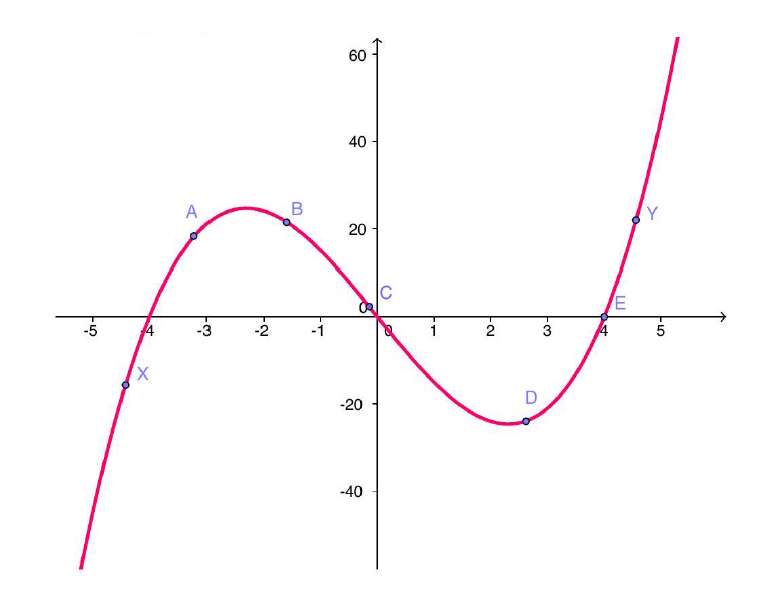
\includegraphics{graph1.PNG}
\caption{graph of \(f(x)\)}
\end{figure}


		\vspace{1em}

		\begin{enumerate}
		\setlength\itemsep{2em}
			\item  $\mathrm{B}$ 
			\item  $\mathrm{C}$ 
			\item  $\mathrm{D}$ 
			\item  $\mathrm{E}$ 
			\item  A 
		\end{enumerate}
	\end{minipage}
	\item
	\begin{minipage}[t]{\linewidth}
		Let \(f(x)=x^{3}-6 x^{2}+10\). At which point(s) on the graph of \(f\)
is the tangent line parallel to the line \(15 x-y=11\) ?


		\vspace{1em}

		\begin{enumerate}
		\setlength\itemsep{2em}
			\item  $(2,-6)$ and $(-2,-22)$ 
			\item  $(5,-15)$ and $(-1,3)$ 
			\item  $(5,-15)$ and $(2,-6)$ 
			\item  $(2,-6)$ and $(-2,22)$ 
		\end{enumerate}
	\end{minipage}
\end{enumerate}




\end{document}
